\documentclass{standalone}

\begin{document}
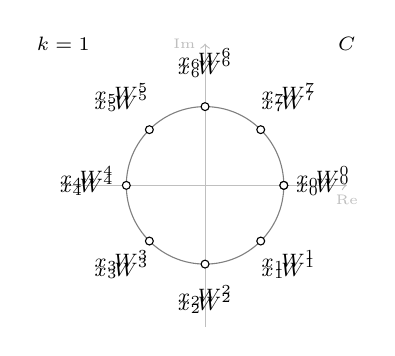
\begin{tikzpicture}
\usetikzlibrary{decorations.pathreplacing,angles,quotes}
\usetikzlibrary{shapes.geometric,shapes.misc}
\usetikzlibrary{calc}

\def\GRIDSIZE{1.8}
\draw[lightgray,->] (0, -\GRIDSIZE) -- (0, \GRIDSIZE)
    node[left] {\tiny Im};
\draw[lightgray,->] (-\GRIDSIZE, 0) -- (\GRIDSIZE, 0)
    node[below] {\tiny Re};
\draw (\GRIDSIZE, \GRIDSIZE) node {\scriptsize $\mathbb C$};

\draw[gray] (0, 0) circle (1);

\draw (-\GRIDSIZE, \GRIDSIZE) node {\scriptsize $k=1$};

\def\N{8}

\foreach \n in {0,...,\N}
{
    \coordinate (Z) at ({cos(-360*\n/\N)}, {sin(-360*\n/\N)});
    \draw[fill=white] (Z) circle (.05);
}


\foreach \n in {0,...,7}
{
    \def\dr{1.5}
    \coordinate (Z) at ({\dr*cos(-360*\n/\N)}, {\dr*sin(-360*\n/\N)});
    \ifthenelse{\n=0 \OR \n=4} {
        \node[yshift=.3em] at (Z) {\scriptsize $x_{\n}\!W^{\n}$};
    }{
        \node at (Z) {\scriptsize $x_{\n}\!W^{\n}$};
    }
}

\end{tikzpicture}
\end{document}

